\chapter{Theoretical overview}
\label{chap:refs}

\section{Introduction}\label{sec:introduction}

The development of a custom Virtual File System (VFS) with versioning and encryption capabilities requires an understanding of several key concepts and technologies.
This chapter aims to provide the necessary background and context to deeper understand the VFS implementation discussed in later chapters.
Even for those already familiar with the subject, a brief refresher on the foundational concepts can be helpful for appreciating design choices made in the VFS solution.

We begin by defining file systems and discussing their critical role in organizing and managing data on various storage devices.
Next, we introduce Virtual File Systems, which serve as a bridge between applications and multiple file systems, and the FUSE library, a key component for implementing our custom VFS solution.
Following that, we delve into the ideal encryption approaches suitable for our use case, focusing on the balance between security, efficiency, and ease of use.
Finally, we discuss the concept of versioning and its significance in managing file history and facilitating data recovery.

\section{File Systems}\label{sec:file-systems}

A file system is a critical component of any operating system, tasked with managing and organizing data stored on a device.
It establishes a structure that enables users to create, read, modify, and delete files and directories, facilitating efficient storage and retrieval of data.
This allows users and applications to interact seamlessly with the underlying storage medium.

There are various types of file systems, each tailored for specific operating systems and purposes.
Notable file systems include NTFS (New Technology File System) for Windows, HFS+ for macOS, and ext4 (fourth extended filesystem) for Linux.
Cross-platform compatibility can be attained using universal file systems like FAT32 or exFAT, which are compatible with multiple operating systems.

File systems employ diverse techniques to organize data, such as partitioning, allocation units, and indexing.
Additionally, file systems manage metadata, which is crucial for organizing and accessing stored data.
Metadata encompasses information such as file names, creation and modification timestamps, file sizes, and access permissions.

\section{Virtual File Systems}\label{sec:virtual-file-systems}

A Virtual File System (VFS) is an essential abstraction layer in modern operating systems, designed to facilitate the interaction between various file systems and user applications.
The VFS functions as an intermediary, enabling applications to access various file systems through a unified interface, regardless of the underlying file system's specific characteristics or structure.

The primary purpose of the VFS is to provide a consistent API for user applications and the kernel, it achieves this abstraction by employing a set of data structures and operations that can be mapped to the corresponding components of different file systems.
Common VFS data structures include superblocks, inodes, dentries, and file objects, which are used to represent file systems, files, directories, and open file instances, respectively.

The VFS plays a critical role in operating system design for several reasons:

\begin{enumerate}
    \item \textbf{File System Independence:} By abstracting file system-specific details, the VFS allows applications to perform operations on files and directories without being aware of the underlying file system.
    This simplifies application development and enables seamless access to different file systems simultaneously.
    \item \textbf{Extensibility:} The VFS framework makes it easier to integrate new file systems into the operating system.
    Developers can implement a file system-specific driver that adheres to the VFS interface, allowing applications to utilize the new file system without any modifications.
    \item \textbf{Interoperability:} With the VFS layer, an operating system can support cross-platform file systems like FAT32 or exFAT, enhancing compatibility among different devices and platforms.
    \item \textbf{Caching and Performance:} The VFS can implement caching strategies and performance optimizations that are applicable across different file systems, improving efficiency and reducing redundant operations.
    \item \textbf{Extensibility:} The VFS can be extended to support additional features, such as encryption and versioning, without the need for kernel modifications.
    That is also the topic of this thesis.
\end{enumerate}

\subsection{VFS Operations}\label{subsec:vfs-operations}

The VFS provides file operations such as creating, reading, writing, and deleting files and directories, but also provides operations for managing file system metadata, such as file permissions and timestamps.
The VFS operations are divided into two categories: \textit{path-based} and \textit{file descriptor-based}.
Path-based operations are used to access files and directories using their absolute or relative paths.
File descriptor-based operations are used to access files and directories using file descriptors, which are unique identifiers assigned to open files and directories.
File descriptors are used to avoid the overhead of resolving paths to file objects, which can be costly for large file systems.

\section{Filesystem in Userspace (FUSE)}\label{sec:filesystem-in-userspace-(fuse)}

FUSE (Filesystem in Userspace) is an open-source software interface that allows developers to create custom file systems in user space without the need for kernel modifications.
It operates by providing a bridge between the kernel's VFS layer and user-space file system implementations.
The kernel communicates with the user-space file system using a well-defined API, allowing developers to create file systems without the need for kernel-level programming.
This abstraction greatly simplifies the development process and reduces the risks associated with kernel modifications.

To implement a FUSE-based file system, developers write a user-space program that registers itself with the FUSE kernel module.
This program defines the required file system operations, such as reading, writing, or listing directories, and handles the communication with the underlying storage medium.
The FUSE kernel module forwards file operation requests from the VFS to the user-space program and returns the results to the VFS layer, effectively creating a seamless interface between the kernel and the user-space file system.

\begin{figure}[ht]
    \centering
    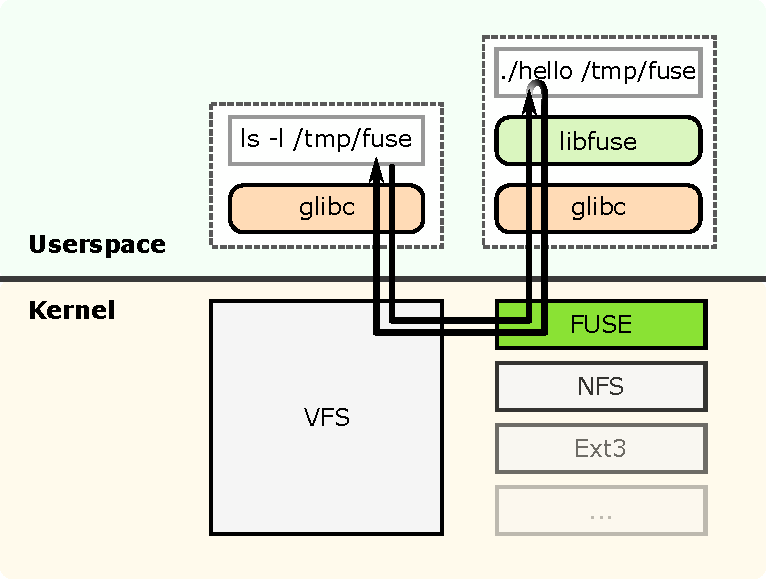
\includegraphics[width=\linewidth]{img/fuse_diagram}
    \caption{FUSE flow-chart diagram}
    \label{fig:fuse-diagram}
\end{figure}

More details about FUSE will be discussed in Chapter\ref{chap:implementation}.

\section{Encryption Approaches}\label{sec:encryption-approaches}

For this use case, an ideal encryption approach should provide strong security while maintaining efficiency and ease of use.
Symmetric key algorithms, such as AES, are well-suited for file-level encryption due to their fast processing speeds and secure key management.
Combining symmetric key encryption with password-based key derivation functions (PBKDFs) ensures that the encryption keys are derived from user-provided passwords, adding an extra layer of security.

\section{Versioning}\label{sec:versioning}

Versioning is a technique used to maintain multiple copies or states of a file or directory, allowing users to access and restore previous versions as needed.
It enables tracking of changes made to files over time, facilitating collaboration and recovery from accidental data loss or corruption.
Implementing versioning in a VFS allows users to take advantage of these benefits without the need for specialized software or manual intervention.



\ldots